\documentclass[11pt,a4paper]{article}
\usepackage[margin=2.1cm]{geometry}
\usepackage[T1]{fontenc}
\usepackage{lmodern}
\usepackage{graphicx}
\usepackage{booktabs}
\usepackage{amsmath}
\usepackage{float}
\usepackage{caption}
\usepackage{subcaption}
\usepackage{enumitem}
\usepackage{microtype}
\usepackage[hidelinks]{hyperref}
\setlist{itemsep=1pt,topsep=3pt}
\captionsetup{font=small}
\graphicspath{{../reports/figures/}}
% generated by make_report_tables.py, do not edit by hand
\newcommand{\nRaw}{48\,842}
\newcommand{\nDup}{52}
\newcommand{\nClean}{48\,790}
\newcommand{\posMarried}{44\%}
\newcommand{\posNotMarried}{7\%}
\newcommand{\posMale}{30.3\%}
\newcommand{\posFemale}{11.1\%}
\newcommand{\husbandMen}{60\%}
\newcommand{\partTimeMen}{12\%}
\newcommand{\partTimeWomen}{27\%}
\newcommand{\capGainZero}{91.9\%}
\newcommand{\capLossZero}{95.4\%}
\newcommand{\nTrain}{29\,274}
\newcommand{\nVal}{9\,758}
\newcommand{\nTest}{9\,758}
\newcommand{\posRate}{23.9\%}
\newcommand{\missWork}{5.7\%}
\newcommand{\missOcc}{5.7\%}
\newcommand{\missCountry}{1.7\%}
\newcommand{\posRateMissOcc}{9.6\%}
\newcommand{\posRatePresentOcc}{24.8\%}
\newcommand{\ablLogRaw}{0.763}
\newcommand{\ablLogEng}{0.774}
\newcommand{\ablLogSd}{0.009}
\newcommand{\ablLogGain}{1.0}
\newcommand{\ablLgbRaw}{0.825}
\newcommand{\ablLgbEng}{0.824}
\newcommand{\ablLgbSd}{0.006}
\newcommand{\ablLgbGain}{-0.1}
\newcommand{\cvDummyNone}{0.239}
\newcommand{\brierDummyNone}{0.182}
\newcommand{\fHalfDummyNone}{0.000}
\newcommand{\fTunedDummyNone}{0.386}
\newcommand{\cvLogNone}{0.774}
\newcommand{\brierLogNone}{0.101}
\newcommand{\fHalfLogNone}{0.667}
\newcommand{\fTunedLogNone}{0.691}
\newcommand{\cvLogBal}{0.773}
\newcommand{\brierLogBal}{0.126}
\newcommand{\fHalfLogBal}{0.685}
\newcommand{\fTunedLogBal}{0.691}
\newcommand{\cvLogSmote}{0.773}
\newcommand{\brierLogSmote}{0.125}
\newcommand{\fHalfLogSmote}{0.688}
\newcommand{\fTunedLogSmote}{0.694}
\newcommand{\cvRfNone}{0.809}
\newcommand{\brierRfNone}{0.093}
\newcommand{\fHalfRfNone}{0.689}
\newcommand{\fTunedRfNone}{0.717}
\newcommand{\cvRfBal}{0.808}
\newcommand{\brierRfBal}{0.113}
\newcommand{\fHalfRfBal}{0.708}
\newcommand{\fTunedRfBal}{0.718}
\newcommand{\cvRfSmote}{0.799}
\newcommand{\brierRfSmote}{0.104}
\newcommand{\fHalfRfSmote}{0.715}
\newcommand{\fTunedRfSmote}{0.715}
\newcommand{\cvLgbNone}{0.824}
\newcommand{\brierLgbNone}{0.088}
\newcommand{\fHalfLgbNone}{0.711}
\newcommand{\fTunedLgbNone}{0.723}
\newcommand{\cvLgbBal}{0.824}
\newcommand{\brierLgbBal}{0.108}
\newcommand{\fHalfLgbBal}{0.713}
\newcommand{\fTunedLgbBal}{0.725}
\newcommand{\cvLgbSmote}{0.820}
\newcommand{\brierLgbSmote}{0.092}
\newcommand{\fHalfLgbSmote}{0.724}
\newcommand{\fTunedLgbSmote}{0.724}
\newcommand{\remedyLossMax}{1.0}
\newcommand{\tunedCvLog}{0.774}
\newcommand{\defaultCvLog}{0.774}
\newcommand{\tunedValLog}{0.772}
\newcommand{\defaultValLog}{0.771}
\newcommand{\tunedGainLog}{0.1}
\newcommand{\bestTrialLog}{29}
\newcommand{\tunedCvRf}{0.814}
\newcommand{\defaultCvRf}{0.809}
\newcommand{\tunedValRf}{0.812}
\newcommand{\defaultValRf}{0.812}
\newcommand{\tunedGainRf}{0.4}
\newcommand{\bestTrialRf}{24}
\newcommand{\tunedCvLgb}{0.830}
\newcommand{\defaultCvLgb}{0.824}
\newcommand{\tunedValLgb}{0.831}
\newcommand{\defaultValLgb}{0.828}
\newcommand{\tunedGainLgb}{0.5}
\newcommand{\bestTrialLgb}{59}
\newcommand{\bestLogC}{8.36}
\newcommand{\bestLogLoneRatio}{0.957}
\newcommand{\bestLogSolver}{saga}
\newcommand{\bestLogMaxIter}{3000}
\newcommand{\bestLogTol}{0.001}
\newcommand{\nTrialsLog}{30}
\newcommand{\bestRfNEstimators}{250}
\newcommand{\bestRfMaxDepth}{16}
\newcommand{\bestRfMinSamplesLeaf}{4}
\newcommand{\bestRfMaxFeatures}{0.332}
\newcommand{\bestRfMaxSamples}{0.801}
\newcommand{\nTrialsRf}{30}
\newcommand{\bestLgbNEstimators}{1400}
\newcommand{\bestLgbLearningRate}{0.0202}
\newcommand{\bestLgbNumLeaves}{14}
\newcommand{\bestLgbMinChildSamples}{31}
\newcommand{\bestLgbSubsample}{0.934}
\newcommand{\bestLgbColsampleBytree}{0.418}
\newcommand{\bestLgbRegLambda}{0.00294}
\newcommand{\bestLgbRegAlpha}{0.0507}
\newcommand{\bestLgbSubsampleFreq}{1}
\newcommand{\nTrialsLgb}{60}
\newcommand{\lgbImpOneName}{reg\_alpha}
\newcommand{\lgbImpOne}{0.25}
\newcommand{\lgbImpTwoName}{colsample\_bytree}
\newcommand{\lgbImpTwo}{0.23}
\newcommand{\brierCalRaw}{0.0873}
\newcommand{\eceCalRaw}{0.008}
\newcommand{\brierCalWeights}{0.1085}
\newcommand{\eceCalWeights}{0.105}
\newcommand{\brierCalPlatt}{0.0872}
\newcommand{\eceCalPlatt}{0.006}
\newcommand{\brierCalIso}{0.0873}
\newcommand{\eceCalIso}{0.008}
\newcommand{\meanPredRaw}{23.9\%}
\newcommand{\meanPredWeights}{34.4\%}
\newcommand{\obsRate}{23.9\%}
\newcommand{\testPrAuc}{0.837}
\newcommand{\testPrAucLow}{0.825}
\newcommand{\testPrAucHigh}{0.848}
\newcommand{\testRocAuc}{0.932}
\newcommand{\testRocAucLow}{0.927}
\newcommand{\testRocAucHigh}{0.937}
\newcommand{\testFOne}{0.738}
\newcommand{\testFOneLow}{0.723}
\newcommand{\testFOneHigh}{0.750}
\newcommand{\testPrecision}{0.686}
\newcommand{\testPrecisionLow}{0.669}
\newcommand{\testPrecisionHigh}{0.703}
\newcommand{\testRecall}{0.798}
\newcommand{\testRecallLow}{0.781}
\newcommand{\testRecallHigh}{0.813}
\newcommand{\testAcc}{0.864}
\newcommand{\testAccLow}{0.857}
\newcommand{\testAccHigh}{0.870}
\newcommand{\testBrier}{0.086}
\newcommand{\testBrierLow}{0.082}
\newcommand{\testBrierHigh}{0.089}
\newcommand{\testEce}{0.011}
\newcommand{\testEceLow}{0.009}
\newcommand{\testEceHigh}{0.018}
\newcommand{\testThr}{0.34}
\newcommand{\brierNoSkill}{0.182}
\newcommand{\brierSkill}{0.53}
\newcommand{\prevalenceTest}{23.9\%}
\newcommand{\tprFemaleBefore}{0.704}
\newcommand{\fprFemaleBefore}{0.038}
\newcommand{\precFemaleBefore}{0.686}
\newcommand{\thrFemaleBefore}{0.34}
\newcommand{\tprMaleBefore}{0.814}
\newcommand{\fprMaleBefore}{0.165}
\newcommand{\precMaleBefore}{0.686}
\newcommand{\thrMaleBefore}{0.34}
\newcommand{\tprFemaleAfter}{0.775}
\newcommand{\fprFemaleAfter}{0.060}
\newcommand{\precFemaleAfter}{0.600}
\newcommand{\thrFemaleAfter}{0.24}
\newcommand{\tprMaleAfter}{0.804}
\newcommand{\fprMaleAfter}{0.159}
\newcommand{\precMaleAfter}{0.691}
\newcommand{\thrMaleAfter}{0.35}
\newcommand{\tprFemaleNoSex}{0.725}
\newcommand{\fprFemaleNoSex}{0.041}
\newcommand{\precFemaleNoSex}{0.673}
\newcommand{\thrFemaleNoSex}{0.35}
\newcommand{\tprMaleNoSex}{0.805}
\newcommand{\fprMaleNoSex}{0.160}
\newcommand{\precMaleNoSex}{0.689}
\newcommand{\thrMaleNoSex}{0.35}
\newcommand{\nFemaleTest}{3\,232}
\newcommand{\nMaleTest}{6\,526}
\newcommand{\posFemaleTest}{338}
\newcommand{\prevFemaleTest}{10.5\%}
\newcommand{\prevMaleTest}{30.6\%}
\newcommand{\rocFemale}{0.950}
\newcommand{\rocMale}{0.915}
\newcommand{\eceFemale}{0.008}
\newcommand{\eceMale}{0.017}
\newcommand{\gapBefore}{0.110}
\newcommand{\gapLowBefore}{0.063}
\newcommand{\gapHighBefore}{0.160}
\newcommand{\accBefore}{0.864}
\newcommand{\fOneBefore}{0.738}
\newcommand{\fprGapBefore}{0.127}
\newcommand{\dpRatioBefore}{0.30}
\newcommand{\gapAfter}{0.029}
\newcommand{\gapLowAfter}{-0.019}
\newcommand{\gapHighAfter}{0.078}
\newcommand{\accAfter}{0.861}
\newcommand{\fOneAfter}{0.733}
\newcommand{\fprGapAfter}{0.098}
\newcommand{\dpRatioAfter}{0.38}
\newcommand{\gapNoSex}{0.080}
\newcommand{\gapLowNoSex}{0.030}
\newcommand{\gapHighNoSex}{0.132}
\newcommand{\accNoSex}{0.864}
\newcommand{\fOneNoSex}{0.736}
\newcommand{\fprGapNoSex}{0.119}
\newcommand{\dpRatioNoSex}{0.31}
\newcommand{\gapPointsBefore}{11.0}
\newcommand{\gapPointsAfter}{2.9}
\newcommand{\extraWomenContacted}{90}
\newcommand{\extraWomenEligible}{24}
\newcommand{\extraWomenShare}{27\%}
\newcommand{\targetTpr}{0.794}
\newcommand{\meanPredFemale}{10.7\%}
\newcommand{\observedFemale}{10.5\%}
\newcommand{\meanPredMale}{30.4\%}
\newcommand{\observedMale}{30.6\%}
\newcommand{\shapOneName}{age}
\newcommand{\shapOne}{0.82}
\newcommand{\shapTwoName}{is\_married}
\newcommand{\shapTwo}{0.64}
\newcommand{\shapThreeName}{education-num}
\newcommand{\shapThree}{0.52}
\newcommand{\shapFourName}{marital-status}
\newcommand{\shapFour}{0.40}
\newcommand{\shapFiveName}{occupation}
\newcommand{\shapFive}{0.34}
\newcommand{\shapSixName}{capital-gain}
\newcommand{\shapSix}{0.33}
\newcommand{\permOneName}{capital-gain}
\newcommand{\permOne}{0.24}
\newcommand{\permTwoName}{marital-status}
\newcommand{\permTwo}{0.10}
\newcommand{\permThreeName}{education-num}
\newcommand{\permThree}{0.06}
\newcommand{\finalName}{without recalibration}
\newcommand{\valPrAucFinal}{0.831}
\newcommand{\valBrierFinal}{0.0873}
\newcommand{\localTpP}{1.00}
\newcommand{\personTpAge}{32}
\newcommand{\personTpHours}{50}
\newcommand{\personTpGain}{15\,024}
\newcommand{\localTpCapitalGain}{+3.93}
\newcommand{\localTpLogCapitalNet}{+2.73}
\newcommand{\localTpEducationNum}{+1.43}
\newcommand{\localTpIsMarried}{+0.45}
\newcommand{\localTpWorkclass}{+0.36}
\newcommand{\localTpAge}{+0.36}
\newcommand{\localFnP}{0.19}
\newcommand{\personFnAge}{27}
\newcommand{\personFnHours}{45}
\newcommand{\personFnGain}{0}
\newcommand{\localFnIsMarried}{+0.63}
\newcommand{\localFnAge}{$-$0.51}
\newcommand{\localFnOccupation}{+0.41}
\newcommand{\localFnMaritalStatus}{+0.41}
\newcommand{\localFnHoursPerWeek}{+0.29}
\newcommand{\localFnWorkclass}{$-$0.29}
\newcommand{\localFpP}{0.50}
\newcommand{\personFpAge}{37}
\newcommand{\personFpHours}{70}
\newcommand{\personFpGain}{0}
\newcommand{\localFpEducationNum}{+1.30}
\newcommand{\localFpOccupation}{+0.71}
\newcommand{\localFpIsMarried}{$-$0.53}
\newcommand{\localFpAge}{+0.52}
\newcommand{\localFpHoursPerWeek}{+0.45}
\newcommand{\localFpWorkclass}{+0.33}
\newcommand{\localBlP}{0.34}
\newcommand{\personBlAge}{57}
\newcommand{\personBlHours}{40}
\newcommand{\personBlGain}{0}
\newcommand{\localBlAge}{+0.86}
\newcommand{\localBlIsMarried}{+0.76}
\newcommand{\localBlMaritalStatus}{+0.46}
\newcommand{\localBlEducationNum}{$-$0.36}
\newcommand{\localBlRelationship}{+0.19}
\newcommand{\localBlLogCapitalNet}{$-$0.14}
\newcommand{\pairedNoSex}{3.0}
\newcommand{\pairedNoSexLow}{1.5}
\newcommand{\pairedNoSexHigh}{4.6}
\newcommand{\pairedGroup}{8.1}
\newcommand{\pairedGroupLow}{5.5}
\newcommand{\pairedGroupHigh}{11.0}
\newcommand{\gapValBefore}{0.076}
\newcommand{\maxValGain}{0.3}
\newcommand{\trainPrAuc}{0.857}
\newcommand{\confTp}{1\,864}
\newcommand{\confFp}{854}
\newcommand{\confFn}{472}
\newcommand{\confTn}{6\,568}
\newcommand{\confPositives}{2\,336}
\newcommand{\confFlagged}{2\,718}
\newcommand{\nRuns}{145}
\newcommand{\nOptunaRuns}{120}


\newcommand{\repo}{\url{https://github.com/LelukDev/applied-ml-adult-group3}}
\newcommand{\tablefile}[1]{\begin{center}\small\resizebox{\linewidth}{!}{\input{generated/#1}}\end{center}}

\title{\vspace{-1.2cm}Predicting income above 50K on the UCI Adult dataset\\[3pt]
\large Applied ML: Foundations, Engineering \& Evaluation, final project of group 3}
\author{Josha\"{\i} Bensoussan \and Lucas Noury \and Elie Maarek}
\date{Albert School, Fall 2026 \quad Code: \repo}

\begin{document}
\maketitle
\vspace{-0.8cm}
\begin{center}
\fbox{\parbox{0.94\textwidth}{\textbf{Dataset used:} UCI Adult (census income), \nRaw{} people from the 1994 US census, loaded with \texttt{fetch\_openml(name="adult", version=2)}. Target: income above 50K (\posRate{} of the people). Sensitive attribute audited: sex.}}
\end{center}

\begin{abstract}
\noindent We build and evaluate a model that predicts whether a person earns more than 50K a year. We compare a logistic regression, a random forest and LightGBM with the same 5-fold stratified cross-validation, and we test three ways of handling the class imbalance. Each model is tuned with Optuna. The final model is the tuned LightGBM (\finalName). On a test set used once, it reaches a PR-AUC of \testPrAuc{} (no-skill baseline \prevalenceTest) and an F1 of \testFOne{}, and its probabilities are well calibrated (ECE \testEce{} on the test set). At one common threshold, women who earn more than 50K are found less often than men (recall \tprFemaleBefore{} against \tprMaleBefore). Removing the sex column helps only a little. Group-specific thresholds chosen on validation reduce the gap from \gapPointsBefore{} to \gapPointsAfter{} points, at a small cost in accuracy.
\end{abstract}

\section{Business problem and data}
We take the point of view of a retail bank that wants to offer a premium product to people who earn more than 50K a year, using only socio-demographic information (no payslip). An eligible person who is missed means lost revenue and an unfair refusal. A wrong offer means a wasted contact. Both errors matter. We rank people with PR-AUC and choose an operating point with F1. We also check that the probabilities can be trusted (calibration) and that the errors are not concentrated on one group (fairness).

The data have 14 variables: six numeric (age, fnlwgt, education-num, capital-gain, capital-loss, hours-per-week) and eight categorical (workclass, education, marital-status, occupation, relationship, race, sex, native-country). One row is one person.

\section{Exploratory analysis and split (requirement 1)}\label{sec:eda}
\subsection{Framing and leakage audit}
The model estimates $P(\text{income} > 50\text{K} \mid \text{profile})$ for one person. Table~\ref{tab:audit} lists what each group of variables means at prediction time. The file has no date and no person identifier, so we cannot make a time split or a group split. We assume that the rows are independent, which is a limit of the data.

\begin{table}[!t]
\centering\small
\begin{tabular}{p{3.3cm}p{3.1cm}p{7.3cm}}
\toprule
Variables & Known at prediction? & Risk and decision \\
\midrule
age, sex, race, native-country & Yes (declared) & Low risk. Sex and race are sensitive: we audit them in Section~\ref{sec:fair}. \\
education, marital-status, relationship & Yes & Medium risk. \texttt{relationship} (Husband, Wife) is a proxy of sex. \texttt{education} is the same information as \texttt{education-num}, so we drop it. \\
workclass, occupation, hours-per-week & Yes & Low risk. Kept. \\
capital-gain, capital-loss & Yes & Medium risk: they are close to an income, so they are almost a consequence of the target. Kept and discussed. \\
fnlwgt & Not a property of the person & It is a census sampling weight. Dropped. \\
\bottomrule
\end{tabular}
\caption{Leakage audit of the variables.}\label{tab:audit}
\end{table}

\subsection{What the data look like}
All statistics in this section use the training set only, so the test set has no influence on our choices.
\begin{itemize}
\item \nDup{} rows are exact duplicates. We remove them before splitting, so that the same record cannot be in the training and in the test set. This leaves \nClean{} people.
\item Missing values (coded ``?'') appear in workclass (\missWork), occupation (\missOcc) and native-country (\missCountry). Workclass and occupation are missing for almost the same people. These people are not like the others: the share above 50K is \posRateMissOcc{} when the occupation is missing, against \posRatePresentOcc{} otherwise. Missing is therefore informative, and we keep it as its own category instead of replacing it with the most frequent value.
\item Capital gain is zero for \capGainZero{} of the people and capital loss for \capLossZero. Both have a long tail.
\item The share above 50K is \posMale{} for men and \posFemale{} for women, and \posMarried{} for married people against \posNotMarried{} for the others. The variable \texttt{relationship} is almost a copy of sex: \husbandMen{} of the men are ``Husband'' and almost no woman is. Women also work part-time (less than 35 hours) more often than men (\partTimeWomen{} against \partTimeMen). These points matter again in Section~\ref{sec:fair}.
\end{itemize}

\begin{figure}[H]
\centering
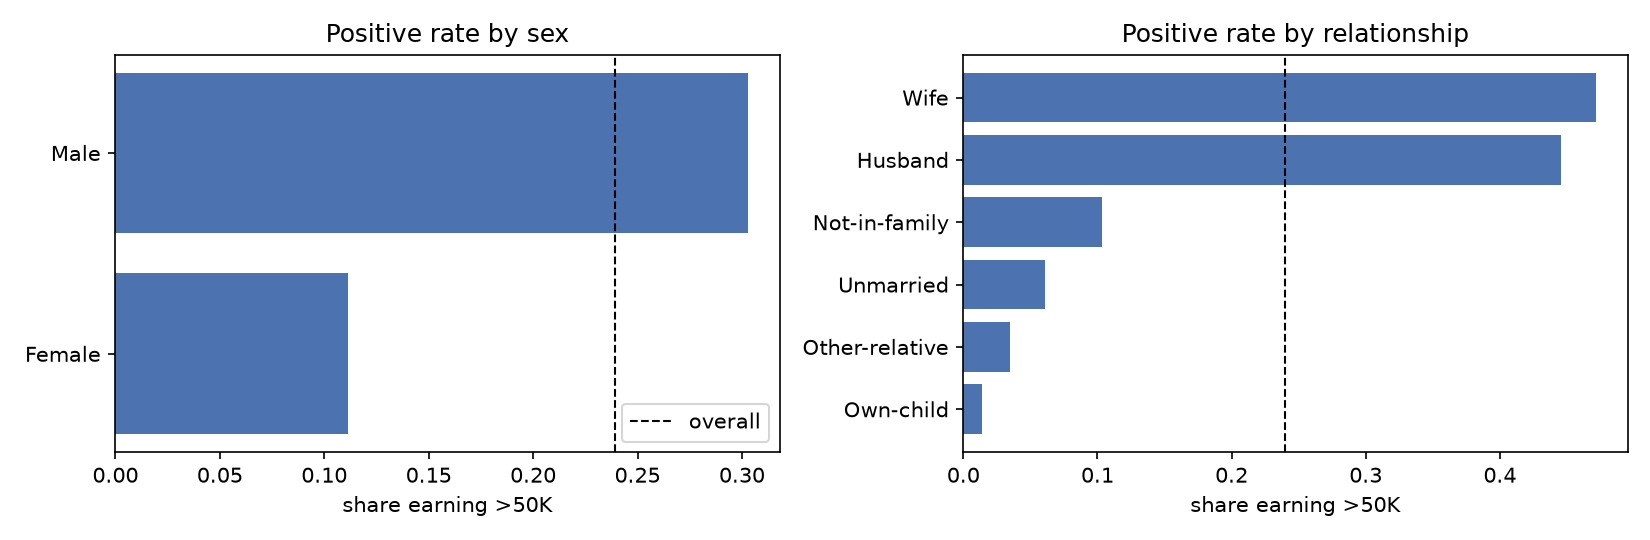
\includegraphics[width=0.7\linewidth]{eda_positive_rate_sex_relationship.png}
\caption{Share of people above 50K by sex and by relationship (training set). The dashed line is the overall rate.}
\end{figure}

\subsection{Split and baseline}
We split the \nClean{} people once, with stratification on the target and seed 42 (Table~\ref{tab:split}). Before the split, rows are sorted, so the result does not depend on the order of the data source. We checked that the OpenML data and the csv copy in the repository give exactly the same split. The training set is used for fitting, cross-validation, Optuna and the choice of the model family. The validation set is used for the calibration method, the decision threshold and the fairness thresholds. The test set is used once at the end. No choice (features, model, hyperparameters, threshold, calibration, fairness thresholds) uses the test set.

\begin{table}[H]
\centering\small
\begin{tabular}{lrr}
\toprule
Split & People & Share >50K \\
\midrule
train & 29\,274 & 23.9\% \\
val & 9\,758 & 23.9\% \\
test & 9\,758 & 23.9\% \\
\bottomrule
\end{tabular}

\caption{Stratified split.}\label{tab:split}
\end{table}

About three people out of four are at most 50K, so accuracy is a poor metric: a model that always answers ``at most 50K'' is right for three people out of four and finds nobody. Our no-skill baseline always predicts the training prevalence. Its PR-AUC is the prevalence (\cvDummyNone), and its Brier score is \brierNoSkill{} on the test set.

\section{Feature engineering (requirement 2)}
Categorical variables are one-hot encoded, with rare levels (fewer than 30 people) grouped together. Numeric variables are standardised. Missing categories become the level ``Missing''. We create five variables:
\begin{enumerate}
\item \texttt{log\_capital\_net} and \texttt{has\_capital}: a signed logarithm of capital gain minus capital loss, and a flag for any capital income. The raw variables are mostly zeros with a long tail, so a linear model cannot use them well.
\item \texttt{is\_married}: one flag for civil or armed-forces spouse, instead of seven marital statuses. It carries a strong signal (\posMarried{} against \posNotMarried{}).
\item \texttt{overtime\_hours}: hours above 40. The effect of hours is not linear around the usual week.
\item \texttt{is\_us}: native-country has 41 levels and most have few people.
\end{enumerate}
We drop \texttt{fnlwgt} and \texttt{education} for the reasons in Table~\ref{tab:audit}.

To check that the new variables help, we compare raw and engineered variables with the same 5-fold cross-validation (Table~\ref{tab:ablation}). For the logistic regression, the PR-AUC goes from \ablLogRaw{} to \ablLogEng{} (+\ablLogGain{} points, fold standard deviation \ablLogSd). For LightGBM, it goes from \ablLgbRaw{} to \ablLgbEng{}, which is within the fold standard deviation (\ablLgbSd). Trees find thresholds and interactions by themselves. We keep the new variables because they help the linear model and cost nothing for the trees.

\begin{table}[H]
\centering\small
\begin{tabular}{llrrr}
\toprule
Model & Features & CV PR-AUC & sd & CV ROC-AUC \\
\midrule
Logistic regression & raw & 0.763 & 0.009 & 0.905 \\
Logistic regression & engineered & 0.774 & 0.007 & 0.908 \\
LightGBM & raw & 0.825 & 0.006 & 0.926 \\
LightGBM & engineered & 0.824 & 0.006 & 0.926 \\
\bottomrule
\end{tabular}

\caption{Raw against engineered variables (5-fold CV on the training set, default hyperparameters).}\label{tab:ablation}
\end{table}

\section{Class imbalance and models (requirements 3, 4 and 5)}
\paragraph{Metrics.} PR-AUC (average precision) is our main metric for ranking, because the positive class is the minority. ROC-AUC is a complement. F1, precision and recall are computed at a threshold. Brier score and ECE measure the quality of the probabilities. Accuracy is only for reference.

\paragraph{Three remedies.} We compare (a) nothing, (b) class weights (\texttt{class\_weight="balanced"}), and (c) SMOTE inside the training folds, through an \texttt{imblearn} pipeline so that synthetic people never reach a validation fold. For each one we choose the threshold that maximises F1 on out-of-fold training predictions, and we apply it unchanged to the validation set.

\paragraph{One Pipeline.} Every candidate is one Pipeline: feature creation, scaling and encoding, then the model. The same object is cross-validated, tuned, calibrated, explained and saved, and it is refitted on the training folds only during cross-validation.

\tablefile{table_models.tex}
\captionof{table}{Three models and three imbalance strategies, default hyperparameters. CV is 5-fold on the training set. ``Tuned thr.'' is the F1-optimal threshold from out-of-fold training predictions. All other columns are on the validation set except the first.}\label{tab:models}

\paragraph{What each step buys.} Going from no skill to a linear model is the biggest jump: PR-AUC goes from \cvDummyNone{} to \cvLogNone. The random forest reaches \cvRfNone{} and LightGBM \cvLgbNone. Trees probably gain from non-linear effects and interactions, but we did not test which ones.

\paragraph{What the remedies change.} None of the three remedies improves the ranking: the PR-AUC is never higher than without a remedy, and it is lower by up to \remedyLossMax{} points. With \posRate{} of positives, the problem is only moderately imbalanced. Class weights raise the Brier score of LightGBM from \brierLgbNone{} to \brierLgbBal, and SMOTE to \brierLgbSmote, so they make the probabilities worse. Tuning the threshold alone is enough for F1: LightGBM without a remedy goes from \fHalfLgbNone{} at 0.5 to \fTunedLgbNone{} with the tuned threshold. This is close to SMOTE at 0.5 (\fHalfLgbSmote) and better than class weights at 0.5 (\fHalfLgbBal). SMOTE also mixes one-hot columns and creates ``half-married'' people. SMOTENC would avoid this, but SMOTE brought no gain in ranking, so we did not try it.

Decision: we do not reweight or resample. The models are trained on the true class mix, and the threshold is tuned on held-out data. This keeps usable probabilities, which a bank needs to estimate the value of a contact.

\section{Hyperparameter tuning and run log (requirements 6 and 7)}
\paragraph{Setup.} We run one Optuna study per model with the TPE sampler (seed 42). One trial is one set of hyperparameters scored by the mean PR-AUC over the same 5 stratified folds of the training set. The whole Pipeline is refitted in each fold. The search spaces are in Appendix C. The best score of a study is optimistic, because the same folds chose the winner. This is why we also report validation scores and a test score. We did not use nested cross-validation: with a test set of \nTest{} people that stays untouched, the final estimate is precise enough.



\tablefile{table_tuned.tex}
\captionof{table}{Default against tuned hyperparameters. CV is on the training set, the other scores are on the validation set.}\label{tab:tuned}

\paragraph{Result.} Tuning helps a little, and more for the more flexible models. The logistic regression gains \tunedGainLog{} points of CV PR-AUC. Its best \texttt{C} is \bestLogC, which is weak regularisation, so its limit is that it is linear and not overfitting. The random forest gains \tunedGainRf{} points and LightGBM \tunedGainLgb{} points. The best LightGBM uses \bestLgbNEstimators{} small trees (\bestLgbNumLeaves{} leaves) and a low learning rate (\bestLgbLearningRate). The gap between model families is larger than the gain from tuning inside a family, so the choice of the model class mattered more than tuning. On the validation set, tuning changes the PR-AUC by at most \maxValGain{} points, which is within the noise between folds. We keep the tuned models because they are not worse. The final family is LightGBM, chosen on the training CV score only.

\begin{figure}[H]
\centering
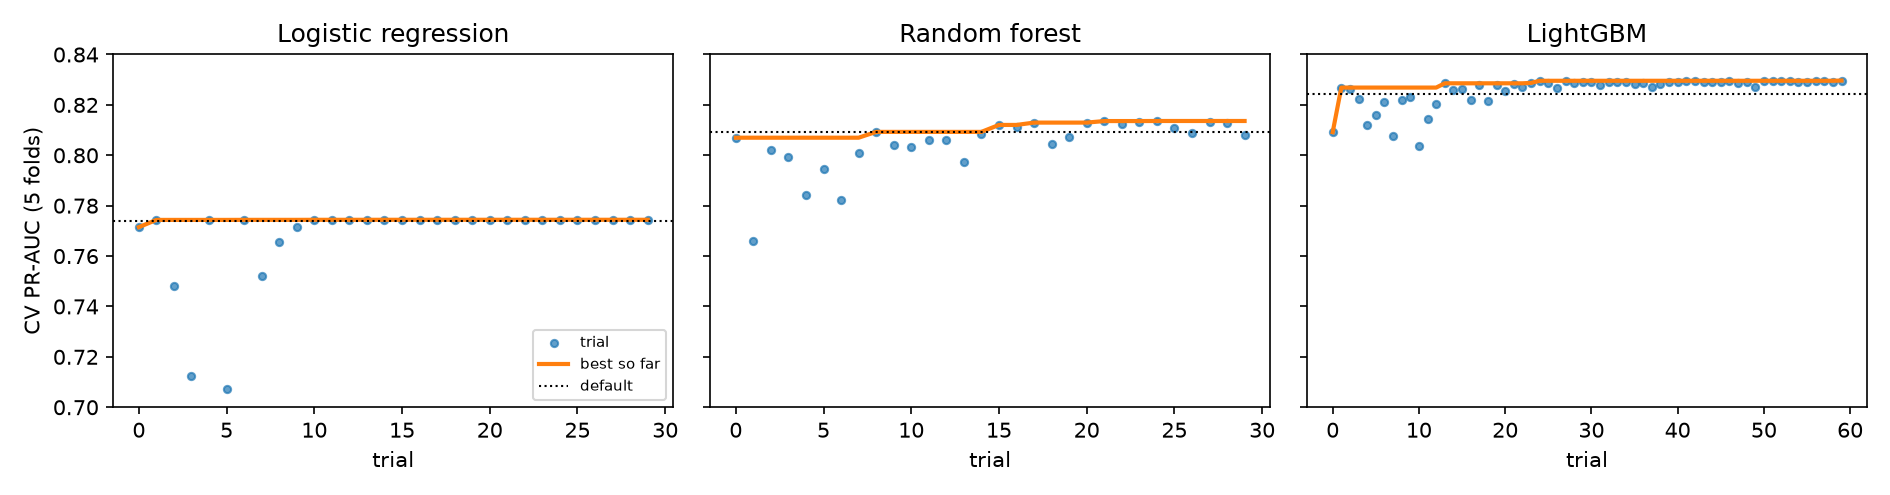
\includegraphics[width=0.8\linewidth]{optuna_history.png}
\caption{CV PR-AUC of each Optuna trial, best score so far, and the default model (dotted line).}
\end{figure}

\paragraph{Run log.} \texttt{runs/run\_log.csv} has one row for each of the \nRuns{} runs: model comparison, feature ablation, each of the \nOptunaRuns{} Optuna trials, tuned models, calibration candidates, final test and fairness policies. The file \texttt{runs/tuning\_log.csv} lists the \nOptunaRuns{} Optuna trials only, with their parameters, fold scores and artifact (the table of trials and the history plot). The best trial of each model is refitted and saved as a model file. The summary is in Appendix~\ref{app:log}. Model files other than the final model are not versioned and are rebuilt by \texttt{run\_all.sh}.

\section{Explainability (requirement 8)}
We use \texttt{shap.TreeExplainer} on the tuned LightGBM, on the validation set, in log-odds units. One-hot columns are summed back into their original variable, which is exact because SHAP values are additive.

\paragraph{Global.} The largest mean absolute SHAP values are for \shapOneName{} (\shapOne), \shapTwoName{} (\shapTwo), \shapThreeName{} (\shapThree), \shapFourName{} (\shapFour), \shapFiveName{} (\shapFive) and \shapSixName{} (\shapSix). Some variables appear twice because they exist in two forms (\texttt{is\_married} and \texttt{marital-status}, \texttt{capital-gain} and \texttt{log\_capital\_net}), and the trees share the signal between them. The directions make business sense: being married, being older, having more education, working in a managerial or professional job, working long hours and having capital income all push towards more than 50K. Sex has a smaller direct effect than marriage and relationship, and most of the difference between men and women goes through these variables.

\begin{figure}[H]
\centering
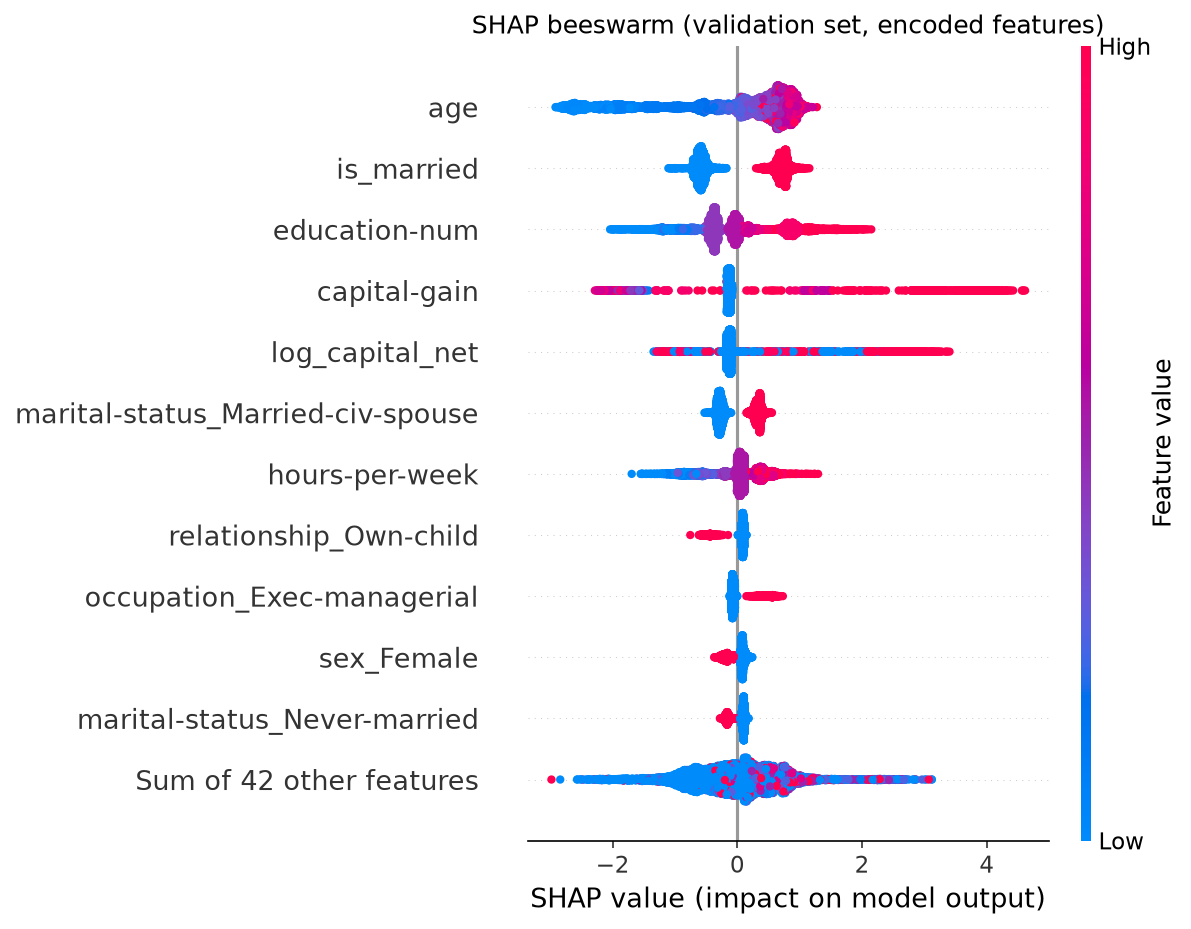
\includegraphics[width=0.48\linewidth]{shap_beeswarm.png}\hfill
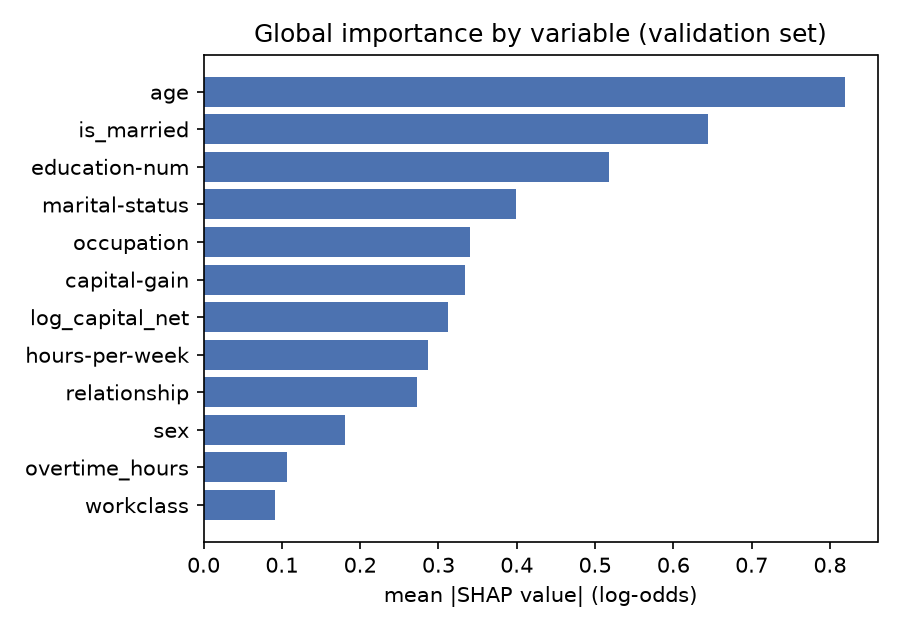
\includegraphics[width=0.48\linewidth]{shap_bar.png}
\caption{Left: SHAP beeswarm (one dot is one person). Right: mean absolute SHAP value by original variable.}
\end{figure}

\paragraph{Permutation importance} (drop in validation PR-AUC when one raw column is shuffled, 10 repeats) answers another question: how much the score depends on a variable. It ranks \permOneName{} first (\permOne), then \permTwoName{} (\permTwo) and \permThreeName{} (\permThree). Capital gain is rare but very strong when present, so shuffling it hurts the ranking a lot, while age moves every prediction a little. Permutation also gives too little credit to correlated variables: \texttt{relationship} costs little when shuffled because \texttt{marital-status} carries the same information.

\paragraph{Individual predictions.} Figure~\ref{fig:local} shows four people from the validation set. (1) The most confident true positive is a \personTpAge-year-old married man with a professional job and a capital gain of \$\personTpGain: capital gain, in its two forms, adds about \localTpCapitalGain{} and \localTpLogCapitalNet{} log-odds. (2) A typical false negative (probability \localFnP, but he earns more than 50K) is a \personFnAge-year-old married, self-employed manager who works \personFnHours{} hours. Marriage (\localFnIsMarried), occupation (\localFnOccupation) and hours (\localFnHoursPerWeek) push up, but his age (\localFnAge) and work class (\localFnWorkclass) pull down. The model sees a young man and misses him. (3) A typical false positive (probability \localFpP, but she earns at most 50K) is a \personFpAge-year-old divorced, self-employed manager with a master's degree who works \personFpHours{} hours. Education (\localFpEducationNum), occupation (\localFpOccupation), age (\localFpAge) and hours (\localFpHoursPerWeek) push up, and only the fact that she is not married (\localFpIsMarried) pulls down. We do not know why she earns less: the data do not say. (4) The person at the threshold (probability \localBlP) is a \personBlAge-year-old married man: age (\localBlAge) and marriage (\localBlIsMarried) push up and education (\localBlEducationNum) pulls down. These are examples, not a proof about all errors, and SHAP explains the model, not the causes of income.

\begin{figure}[H]
\centering
\begin{subfigure}{0.37\linewidth}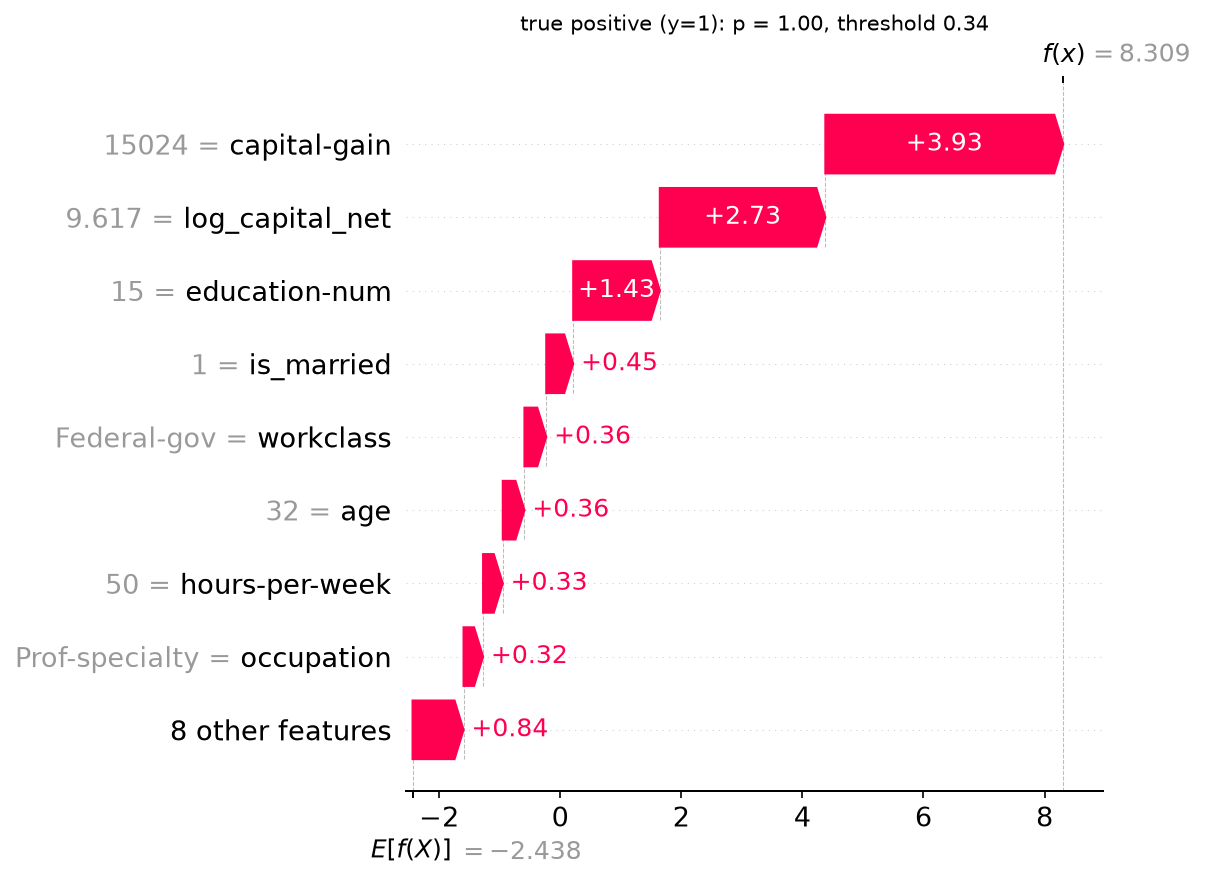
\includegraphics[width=\linewidth]{shap_waterfall_true_positive.png}\caption*{(1) true positive}\end{subfigure}\hfill
\begin{subfigure}{0.37\linewidth}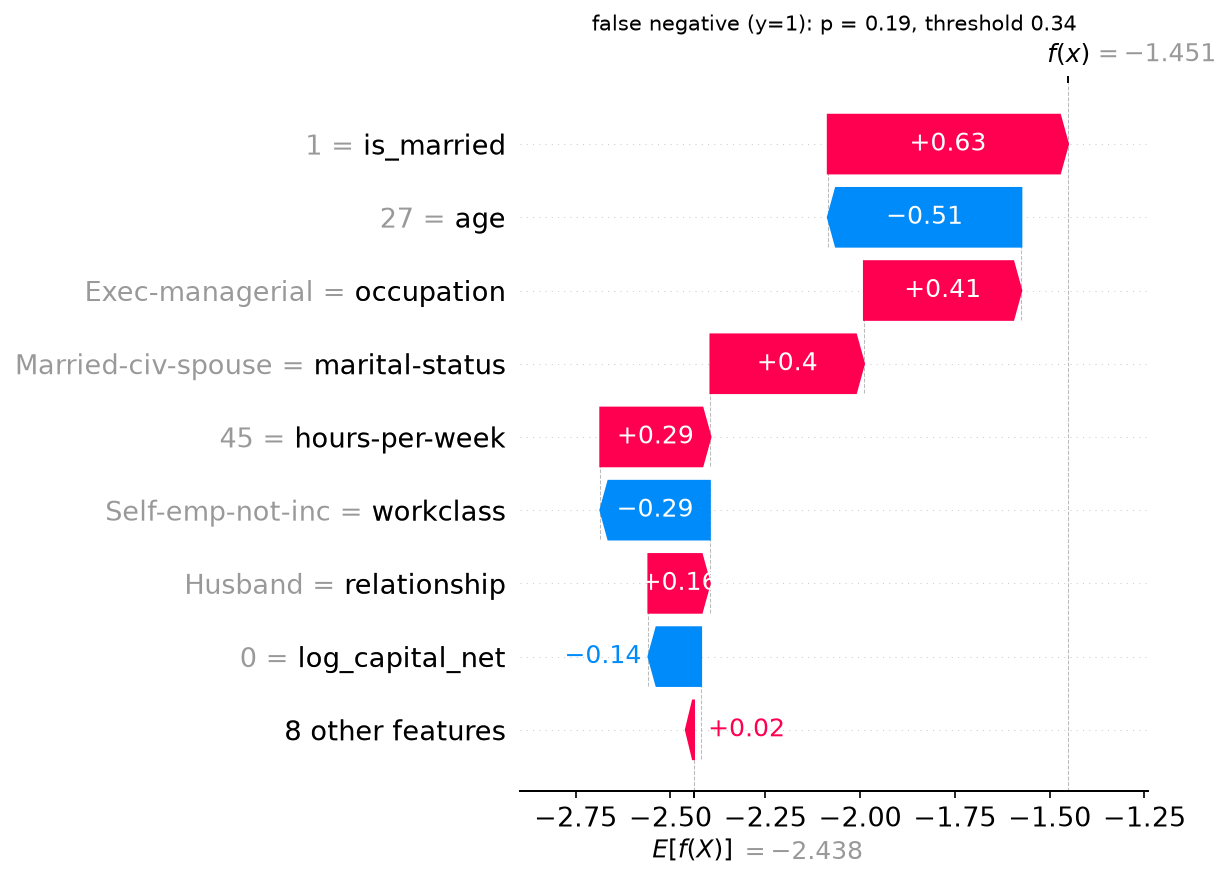
\includegraphics[width=\linewidth]{shap_waterfall_false_negative.png}\caption*{(2) false negative}\end{subfigure}\\[2pt]
\begin{subfigure}{0.37\linewidth}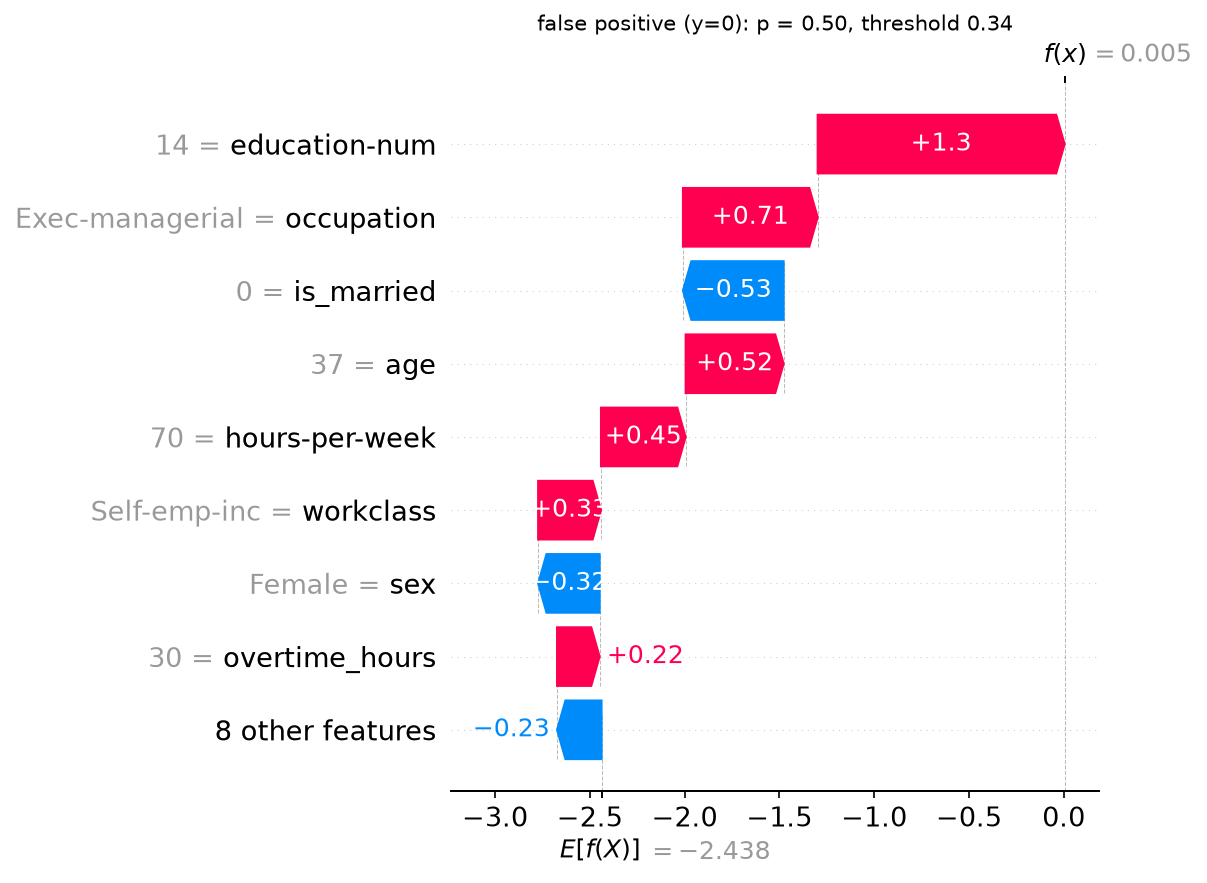
\includegraphics[width=\linewidth]{shap_waterfall_false_positive.png}\caption*{(3) false positive}\end{subfigure}\hfill
\begin{subfigure}{0.37\linewidth}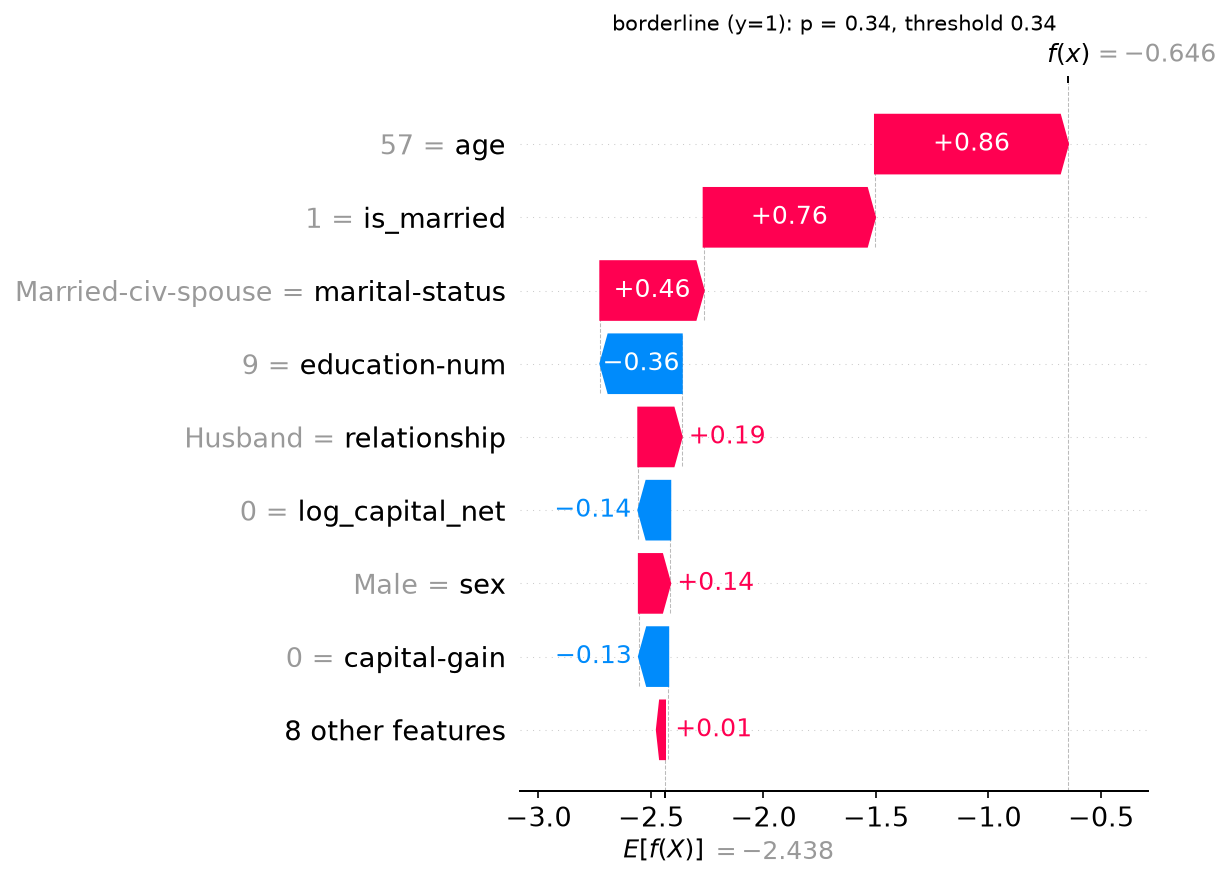
\includegraphics[width=\linewidth]{shap_waterfall_borderline.png}\caption*{(4) at the threshold}\end{subfigure}
\caption{SHAP waterfalls for four people (validation set), in log-odds.}\label{fig:local}
\end{figure}

\section{Calibration (requirement 9)}
We compare four candidates, all fitted on the training set and compared on the validation set: the tuned LightGBM as is, the same with class weights, and Platt scaling and isotonic regression applied with \texttt{CalibratedClassifierCV(cv=5)}. Each calibrator is learned on out-of-fold scores, never on in-sample predictions.

\begin{table}[H]
\centering\small
\begin{tabular}{lrrrr}
\toprule
Candidate & Brier & ECE & PR-AUC & Mean prediction \\
\midrule
LightGBM as is & 0.0873 & 0.0085 & 0.831 & 0.239 \\
with class weights & 0.1085 & 0.1049 & 0.831 & 0.344 \\
Platt scaling & 0.0872 & 0.0060 & 0.831 & 0.239 \\
isotonic regression & 0.0873 & 0.0078 & 0.831 & 0.239 \\
\bottomrule
\end{tabular}

\caption{Calibration candidates on the validation set (ECE with 15 equal-width bins).}\label{tab:cal}
\end{table}

\begin{figure}[H]
\centering
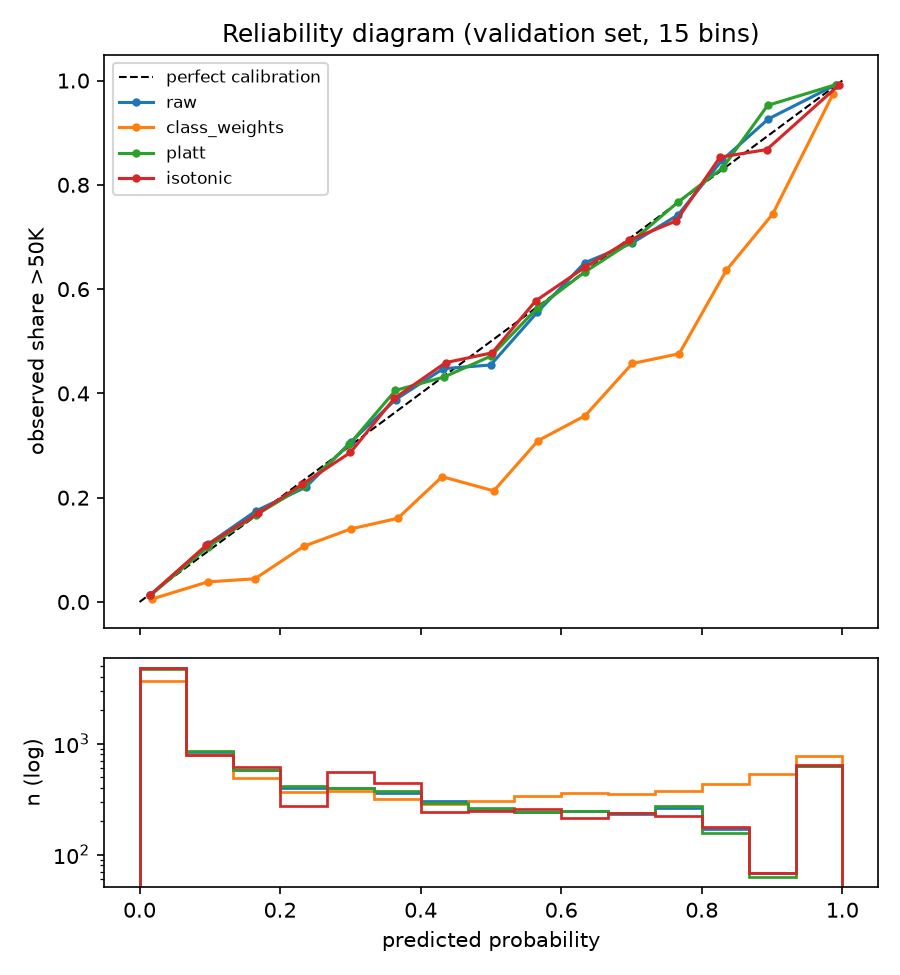
\includegraphics[width=0.46\linewidth]{calibration_reliability.png}
\caption{Reliability diagram (top) and number of predictions per bin on a log scale (bottom).}\label{fig:rel}
\end{figure}

\paragraph{Reading.} LightGBM as is follows the diagonal. Its mean prediction (\meanPredRaw) matches the observed rate (\obsRate), and its ECE is \eceCalRaw. The gaps in the 0.1-wide bins are small and have both signs, so the model is neither over-confident nor under-confident in general. Class weights make the model strongly over-confident: its curve is below the diagonal in every bin, and its mean prediction is \meanPredWeights, because the model was trained as if the positives were half of the data. The ECE goes from \eceCalRaw{} to \eceCalWeights. Platt scaling and isotonic regression give a Brier score within 0.001 of the raw model (\brierCalPlatt{} and \brierCalIso{} against \brierCalRaw), so they bring nothing here. Differences this small are noise, and the course (S8) advises the simpler method in this case. Our rule is to keep the raw model unless a calibrator lowers the Brier score by more than 0.001. The final model is therefore the tuned LightGBM \finalName.

\paragraph{Can we trust the probabilities?} Yes, as they are, for a decision such as estimating the value of a contact. Two cautions: the bins in the middle contain only a few hundred people, so their gaps have about two points of noise, and the calibration holds for the 1994 population. It should be monitored if the data change. Calibration also holds inside each sex (Section~\ref{sec:fair}).

\paragraph{Final test.} The threshold is \testThr, chosen on validation (best F1). The test set is used here for the first time. Table~\ref{tab:test} gives the result with bootstrap intervals (1000 resamples of the test set, model and threshold fixed). PR-AUC is \trainPrAuc{} on the training set, \tunedCvLgb{} in cross-validation, \valPrAucFinal{} on validation and \testPrAuc{} on test. The model fits the training data better than new data, but validation and test agree, and the validation value is inside the test interval, so we see no sign of overfitting to the selection process. The Brier skill score against the no-skill model is \brierSkill. At the threshold, the model finds \confTp{} of the \confPositives{} people above 50K and flags \confFp{} people by mistake (Figure~\ref{fig:curves}). The F1 threshold is only a first choice: a real use needs the value of a conversion and the cost of a contact.

\begin{table}[H]
\centering\small
\begin{tabular}{lrr}
\toprule
Metric & Estimate & 95\% interval \\
\midrule
PR-AUC & 0.837 & [0.825, 0.848] \\
ROC-AUC & 0.932 & [0.927, 0.937] \\
F1 & 0.738 & [0.723, 0.750] \\
Precision & 0.686 & [0.669, 0.703] \\
Recall & 0.798 & [0.781, 0.813] \\
Accuracy & 0.864 & [0.857, 0.870] \\
Brier & 0.086 & [0.082, 0.089] \\
ECE & 0.011 & [0.009, 0.018] \\
\bottomrule
\end{tabular}

\caption{Final model on the test set.}\label{tab:test}
\end{table}

\begin{figure}[H]
\centering
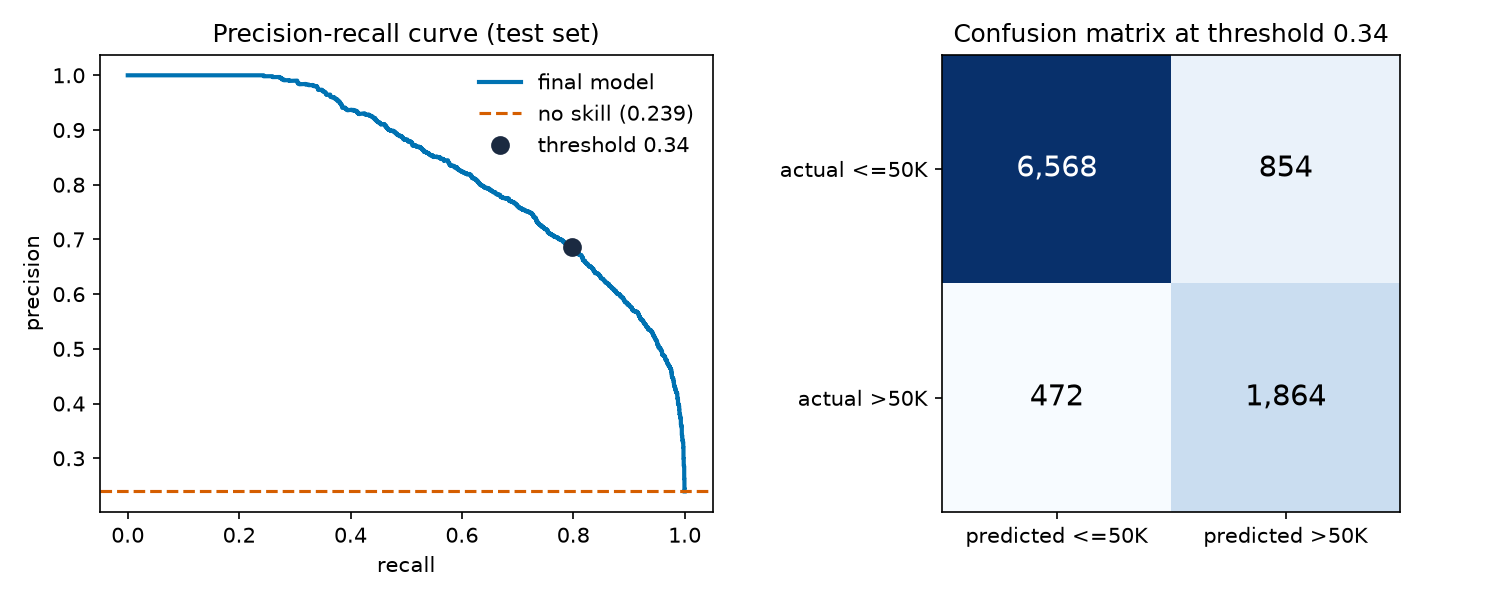
\includegraphics[width=0.75\linewidth]{final_test_curves.png}
\caption{Precision-recall curve and confusion matrix of the final model on the test set.}\label{fig:curves}
\end{figure}

\section{Fairness and bias audit (requirement 10)}\label{sec:fair}
\paragraph{Attribute and definition.} We audit sex. We use equal opportunity: among the people who really earn more than 50K, the chance of being selected should not depend on sex ($\mathrm{TPR}_{\text{men}} = \mathrm{TPR}_{\text{women}}$). We prefer it to demographic parity because the base rates really differ (\prevMaleTest{} of the men and \prevFemaleTest{} of the women are above 50K in the test set). Equal selection rates would mean offering the product to many ineligible women or refusing it to eligible men. We also report the false positive rate gap and the selection-rate ratio, with 95\% bootstrap intervals (1000 resamples of the test set).

\paragraph{Audit.} With one common threshold, eligible women are found \gapPointsBefore{} points less often than eligible men (gap \gapBefore, 95\% interval [\gapLowBefore, \gapHighBefore]). The interval excludes zero. The model ranks women at least as well as men (ROC-AUC \rocFemale{} against \rocMale) and is calibrated in both groups (ECE \eceFemale{} and \eceMale). The problem is the operating point: eligible women get lower scores, so one common cut-off misses more of them. This is probably linked to the points in Section~\ref{sec:eda} (fewer ``Husband'' or ``Wife'', more part-time work), but we did not test it.

\paragraph{First fix: remove the sex column.} We retrain without the variable \texttt{sex}. The gap becomes \gapNoSex{} (interval [\gapLowNoSex, \gapHighNoSex]). On the same resamples of the test set, the gap falls by only \pairedNoSex{} points (95\% interval [\pairedNoSexLow, \pairedNoSexHigh]). Variables such as \texttt{relationship} and marital status probably carry the same information, but we did not test this.

\paragraph{Mitigation: one threshold per sex.} On the validation set we compute the recall of the original policy (\targetTpr) and choose, for each sex, the threshold that gives this recall in that group: \thrFemaleAfter{} for women and \thrMaleAfter{} for men. These thresholds are then fixed and applied to the test set.

\tablefile{table_fair_policies.tex}
\captionof{table}{Before and after on the untouched test set. DP ratio is the selection rate of women divided by the selection rate of men.}\label{tab:fair}

\paragraph{Result.} The gap in recall falls from \gapPointsBefore{} to \gapPointsAfter{} points, and its interval now contains zero. On the same resamples, the thresholds reduce the gap by \pairedGroup{} points (95\% interval [\pairedGroupLow, \pairedGroupHigh]). The accuracy goes from \accBefore{} to \accAfter{} and the F1 from \fOneBefore{} to \fOneAfter, a small cost. The cost is mostly paid in precision for women (\precFemaleBefore{} to \precFemaleAfter): the bank contacts about \extraWomenContacted{} more women in the test set, and \extraWomenEligible{} of them (\extraWomenShare) are eligible. This is a small sample, and these extra contacts are less precise than the average contact for women. The recall of women on the test set (\tprFemaleAfter) is below the target recall (\targetTpr), because the thresholds are estimated on a small validation set. The false positive gap (\fprGapBefore{} to \fprGapAfter) and the demographic parity ratio (\dpRatioBefore{} to \dpRatioAfter) also improve, although we did not target them. The false positive gap stays large, so the model does not satisfy equalised odds.

\begin{figure}[H]
\centering
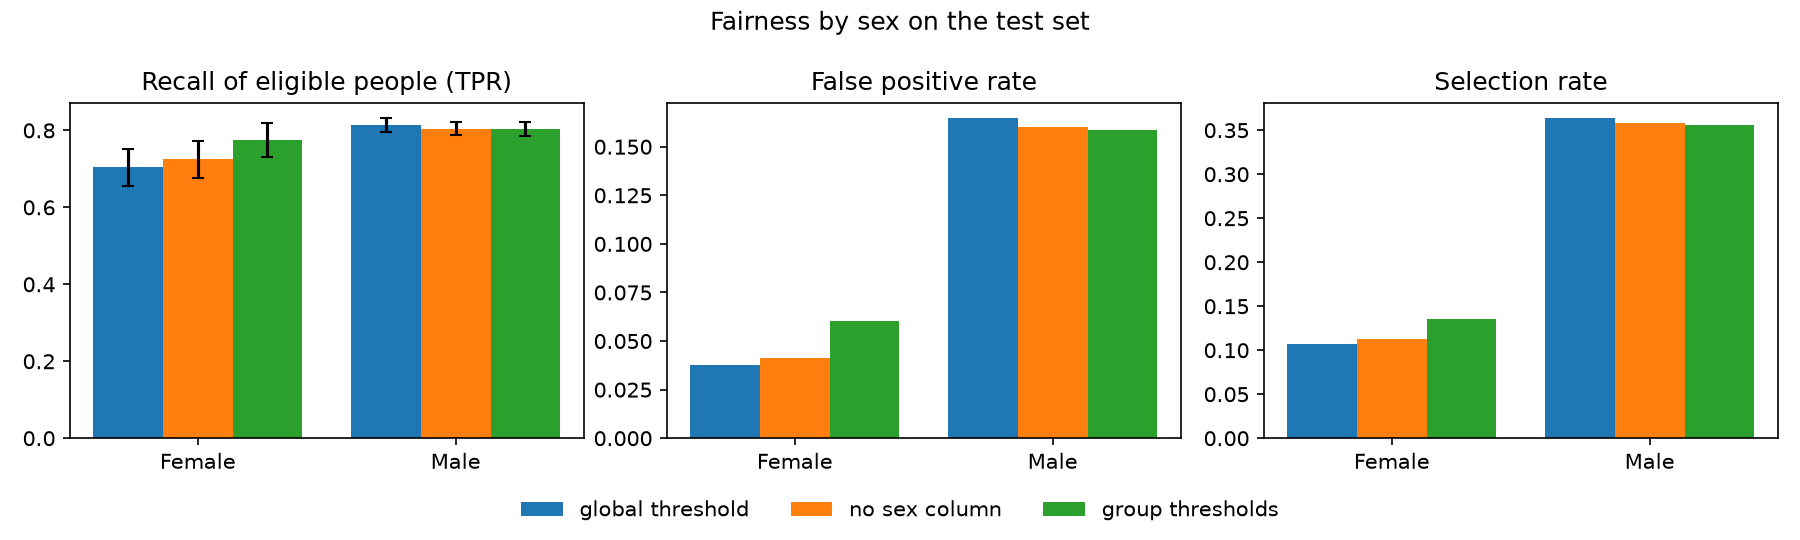
\includegraphics[width=0.78\linewidth]{fairness_sex.png}
\caption{Recall (with 95\% intervals), false positive rate and selection rate by sex for the three policies (test set).}
\end{figure}

\paragraph{Limits.} Using sex at decision time means treating people differently because of their sex (disparate treatment). It may be illegal in some settings (credit decisions, or insurance pricing in the EU), even if it corrects the difference in results between the groups (disparate impact). The labels reflect pay inequality in 1994, and equal opportunity takes them as the truth. The intervals keep the thresholds fixed, so they ignore the uncertainty of estimating the thresholds on the validation set (only a few hundred positive women in each set). The gap at the global threshold is \gapValBefore{} on the validation set and \gapBefore{} on the test set, so the size of the gap itself is uncertain. Race stays a variable of the model and we did not audit it.

\section{Conclusion and limits}
A tuned LightGBM in one Pipeline ranks high earners well (PR-AUC \testPrAuc{} on the test set) with calibrated probabilities, and group thresholds remove most of the recall gap between men and women for a small loss in accuracy. Three lessons:
\begin{itemize}
\item The model family mattered more than hyperparameter tuning.
\item On this moderately imbalanced problem, threshold tuning gives the same F1 as reweighting and keeps the probabilities usable.
\item Dropping the sex column reduced the gap by only \pairedNoSex{} points, because other variables carry similar information.
\end{itemize}

Limits: 1994 data, binary sex, one split and one seed, rows assumed independent, and a census sample is not a bank's customer base. A real use needs the value of a conversion and the cost of a contact to set the threshold, and monitoring of calibration and recall by group.

\newpage
\section*{Contribution statement}
We worked together and helped each other on every part of the project. The main roles were the following. Lucas worked mostly on the analysis: data exploration, models, tuning, explanations, calibration and the fairness audit. Josha\"{\i} worked mostly on the report: its creation, its structure and its format. Elie helped on the analysis and on checking the results.

\section*{Use of AI tools}
For the analysis, we used an AI coding assistant to help us with the code and the visualisations. We chose the topic and the dataset, took the final decisions and checked the results against the result tables. All numbers in this report are generated from the result tables.

\appendix
\section{Run log summary}\label{app:log}
\begin{table}[H]
\centering\small
\begin{tabular}{lrl}
\toprule
Stage & Runs & Content \\
\midrule
compare & 10 & no skill + 3 models x 3 imbalance strategies \\
ablation & 4 & raw vs engineered features \\
optuna & 120 & one row per trial \\
tuned & 3 & best trial of each model, refitted \\
calibration & 4 & calibration candidates \\
final\_test & 1 & final model on the test set \\
fairness & 3 & three decision policies \\
total & 145 &  \\
\bottomrule
\end{tabular}

\caption{Content of \texttt{runs/run\_log.csv}.}
\end{table}

\section{Metrics by sex}
\tablefile{table_fair_groups.tex}
\captionof{table}{Metrics by sex on the test set for the three policies.}

\section{Search spaces}
\begin{table}[H]
\centering\small
\begin{tabular}{lp{10.4cm}r}
\toprule
Model & Search space & Trials \\
\midrule
Logistic regression & C from 0.001 to 100 (log); l1\_ratio from 0 to 1 (elastic net, saga) & \nTrialsLog \\
Random forest & n\_estimators 100 to 500; max\_depth 4 to 40 (log); min\_samples\_leaf 1 to 50 (log); max\_features 0.1 to 0.8; max\_samples 0.5 to 1 & \nTrialsRf \\
LightGBM & n\_estimators 200 to 1500; learning\_rate 0.01 to 0.2 (log); num\_leaves 8 to 128 (log); min\_child\_samples 5 to 200 (log); subsample 0.5 to 1; colsample\_bytree 0.4 to 1; reg\_lambda and reg\_alpha 0.001 to 10 (log) & \nTrialsLgb \\
\bottomrule
\end{tabular}
\caption{Search spaces. The budget follows the size of each space.}
\end{table}

\section{Where to find each requirement}
\begin{table}[H]
\centering\small
\begin{tabular}{lll}
\toprule
Requirement & Code & Section \\
\midrule
1 EDA and split & \texttt{01\_eda.py}, \texttt{get\_splits} in \texttt{common.py} & 2 \\
2 Features & \texttt{add\_features} in \texttt{common.py}, \texttt{02\_compare\_models.py} & 3 \\
3 Class imbalance & \texttt{02\_compare\_models.py} & 4 \\
4 Three models & \texttt{02\_compare\_models.py}, \texttt{06\_final\_test.py} & 4, 7 \\
5 Pipeline & \texttt{build\_pipeline} in \texttt{common.py} & 4 \\
6 Optuna & \texttt{03\_tune\_optuna.py} & 5 \\
7 Run log & \texttt{log\_run} in \texttt{common.py}, \texttt{runs/run\_log.csv} & 5, A \\
8 SHAP & \texttt{04\_explain.py} & 6 \\
9 Calibration & \texttt{05\_calibration.py}, \texttt{06\_final\_test.py} & 7 \\
10 Fairness & \texttt{07\_fairness.py} & 8 \\
Prediction endpoint & \texttt{serve.py} (see the README) & \\
\bottomrule
\end{tabular}
\caption{Requirements and where they are in the repository.}
\end{table}

\end{document}
